% @see : https://coopmaths.fr/alea/?uuid=dnb_2026_01_sujet0va_3&alea=fjpu&uuid=dnb_2024_09_metropole_4&alea=dhH9&uuid=dnb_2022_09_polynesie_4&alea=fEGA&v=eleve&pdfParam=eyJ0aXRsZSI6IiIsInJlZmVyZW5jZSI6IiIsInN1YnRpdGxlIjoiIiwic3R5bGUiOiJDb29wbWF0aHMiLCJmb250T3B0aW9uIjoiU3RhbmRhcmRGb250IiwidGFpbGxlRm9udE9wdGlvbiI6MTIsImR5c1RhaWxsZUZvbnRPcHRpb24iOjE0LCJjb3JyZWN0aW9uT3B0aW9uIjoiQXZlY0NvcnJlY3Rpb24iLCJxcmNvZGVPcHRpb24iOiJTYW5zUXJjb2RlIiwidHlwZUZpY2hlIjoiRmljaGUiLCJkdXJhdGlvbkNhbk9wdGlvbiI6IjkgbWluIiwidGl0bGVPcHRpb24iOiJTYW5zVGl0cmUiLCJuYlZlcnNpb25zIjoxLCJleG9zIjp7fX0\%3D
\documentclass[a4paper,12pt,fleqn]{memoir}
\setlrmarginsandblock{.5cm}{.5cm}{*}
\setulmarginsandblock{.5cm}{.5cm}{*}
 \usepackage{auto-pst-pdf}
%%% COULEURS %%%
\usepackage[table,svgnames]{xcolor}
\definecolor{nombres}{cmyk}{0,.8,.95,0}
\definecolor{gestion}{cmyk}{.75,1,.11,.12}
\definecolor{gestionbis}{cmyk}{.75,1,.11,.12}
\definecolor{grandeurs}{cmyk}{.02,.44,1,0}
\definecolor{geo}{cmyk}{.62,.1,0,0}
\definecolor{algo}{cmyk}{.69,.02,.36,0}
\definecolor{correction}{cmyk}{.63,.23,.93,.06}
% Couleur des filets des tableaux

\usepackage[most]{tcolorbox} % Supprimé à cause de conflits avec ProfCollege
\tcbuselibrary{documentation}

%%%%%%%% Modification paramétrage pour footnotes
% Le paquet semble déjà appelé en amont, curieux qu'il n'y ait pas eu de clash
% avec l'appel ci-dessous mais seulement quand j'ai essayé de l'inclure avec l'option lualatex

% \usepackage{hyperref}
% Parametrages
\hypersetup{
    colorlinks=true,% On active la couleur pour les liens. Couleur par défaut rouge
    linkcolor=black,% On définit la couleur pour les liens internes
    % filecolor=magenta,% On définit la couleur pour les liens vers les fichiers locaux      
    urlcolor=black,% On définit la couleur pour les liens vers des sites web
    % pdftitle={Puissance Quatre},% On définit un titre pour le document pdf
    % pdfpagemode=FullScreen,% On fixe l'affichage par défaut à plein écran
    }
% Pour avoir les numérotations arabic y compris dans les environnements tcolorbox
\renewcommand{\thempfootnote}{\arabic{mpfootnote}}
%%%%%%%%

\usepackage{multicol} 
\usepackage{calc}
\usepackage{enumitem}
\usepackage{graphicx}
\usepackage{tabularx}
%\usepackage{tablvar}

\setlength{\parindent}{0mm}
\renewcommand{\arraystretch}{1.5}
\renewcommand{\labelenumi}{\textbf{\theenumi{}.}}
\renewcommand{\labelenumii}{\textbf{\theenumii{}.}}
\setlength{\fboxsep}{3mm}
 

\setlength{\premulticols}{0pt}

\newcounter{ExoMA}

\newlength{\parindentMA}%
\setlength{\parindentMA}{\parindent} 

\usepackage{simplekv}
 

\usepackage{fancyhdr}
\fancyhead[C]{}
\fancyfoot{}

\def\bla{}
 
 


%%% MISE EN PAGE %%%

\usepackage[margin=1.5cm]{geometry}
\usepackage{setspace}
  \usepackage{eurosym}
\usepackage{pgf}%
\usepackage{pgfplots}
\pgfplotsset{compat=1.18}
\usetikzlibrary{babel,arrows, arrows.meta,calc,fit,patterns,plotmarks,shapes.geometric,shapes.misc,shapes.symbols,shapes.arrows,shapes.callouts, shapes.multipart, shapes.gates.logic.US,shapes.gates.logic.IEC, er, automata,backgrounds,chains,topaths,trees,petri,mindmap,matrix, calendar, folding,fadings,through,positioning,scopes,decorations.fractals,decorations.shapes,decorations.text,decorations.pathmorphing,decorations.pathreplacing,decorations.footprints,decorations.markings,shadows}

\spaceskip=2\fontdimen2\font plus 3\fontdimen3\font minus3\fontdimen4\font\relax %Pour doubler l'espace entre les mots
 
 
  

\usepackage[french]{babel}
% loadPackagesFromContent
\usepackage{pstricks}
\usepackage{pst-plot}
\usepackage{multido}
\usepackage{pst-fun}
\newcommand{\e}{\mathrm{e}}
\usepackage{amsmath}
\usepackage{amssymb}
\usepackage{etoolbox}
\newbool{dys}
\setbool{dys}{false}          
\ifbool{dys}{
% POLICE DYS
% ===== VARIABLE =====
\def\FontChoisie{Fira} % valeurs possibles : Fira, lmodern, tgheros
\newcommand{\choiceFontsDys}[1]{
\ifstrequal{#1}{Fira}{%
  % Fira Sans + Fira Math
  % Description : Fira Sans est une police moderne, et Fira Math est une version mathématique compatible qui maintient le style sans-serif.
  % Utilisation : Fonctionne bien avec XeLaTeX et LuaLaTeX.
  \usepackage{fontspec}
  \setmainfont{Fira Sans}
  \setsansfont{Fira Sans}
  \usepackage{unicode-math}
  \setmathfont{Fira Math}
}{}
\ifstrequal{#1}{lmodern}{%
  % Latin Modern Sans
  % Description : Une version sans-serif de la célèbre police Latin Modern, qui est compatible avec mathastext.
  % Utilisation : Fonctionne avec pdfLaTeX, XeLaTeX et LuaLaTeX.
  \usepackage{lmodern}
  \renewcommand{\familydefault}{\sfdefault}
  \usepackage{mathastext}
}{}
\ifstrequal{#1}{tgheros}{%
  % TeX Gyre Heros + mathastext
  % Description : TeX Gyre Heros est une alternative à Helvetica, et le package mathastext permet d'utiliser la même police pour les mathématiques.
  % Utilisation : Fonctionne avec pdfLaTeX, XeLaTeX, ou LuaLaTeX.
  \usepackage{tgheros}
  \renewcommand{\familydefault}{\sfdefault}
  \usepackage{mathastext}
}{}
}
% Fira ou lmodern ou tgheros
\choiceFontsDys{\FontChoisie}

%\usepackage{unicode-math}
%\usepackage{fontspec}
%\setmainfont{TeX Gyre Schola}
%\setsansfont{TeX Gyre Schola}
%\setmathfont{TeX Gyre Schola Math}
%\setmainfont{OpenDyslexic}[Scale=1.0]
%\setsansfont{OpenDyslexic}[Scale=1.0]
%\setmathfont{OpenDyslexic}[Scale=1.0,range=up/{Latin,latin,num}]
\usepackage[fontsize=14]{scrextend}
\usepackage{setspace}
\setstretch{1.7}
% Une valeur d'environ 1.2 à 1.7 est souvent recommandée. Cela permet d'augmenter l'espace entre les lignes tout en offrant un léger espacement entre les mots.
\setlength{\spaceskip}{1.2em}  
% Une valeur d'environ 1.2em à 1.5em est couramment conseillée. Cela crée un espace plus ample entre les mots, ce qui peut aider à réduire la fatigue visuelle et à améliorer la fluidité de la lecture.
}{
% POLICE STANDARD
\usepackage[T1]{fontenc} 
\usepackage[scaled=1]{helvet}
\usepackage[fontsize=13]{scrextend}
}
\begin{document}
\pagestyle{empty}
\begin{center}{\textbf{{\Huge \center Contrôle chapitres 7 et 8}\\
On prendra soin de rédiger correctement.}.}\end{center}
\subsection*{Exercice 1 - 6 points} 
\begin{tikzpicture}[baseline,scale = 0.5]

    \tikzset{
      point/.style={
        thick,
        draw,
        cross out,
        inner sep=0pt,
        minimum width=5pt,
        minimum height=5pt,
      },
    }
    \clip (-13,-6) rectangle (1,9);
    	\draw  [line width = 2,preaction={fill,opacity = 1}] (-6.354802039468767,4.706967815340633) -- (-4.8,3.8) -- (-5.836716358379734,2.3285316203642488) arc (-125.17:-210.26:1.8) ;
	\draw  [line width = 2,preaction={fill,opacity = 1}] (-1.5547528974661722,1.907052053534163) -- (0,1) -- (-1.5802120312458918,0.13806616477496814) arc (-151.39:-210.26:1.8) ;
	\draw  [color={black},line width = 2,preaction={fill,opacity = 1}] (-4.321025070400122,-1.3568317752135426) -- (-5.5,-2) -- (-6.231918999775239,-0.873970769576556) arc (123.02:28.61:1.34) ;
	\draw[color={black}] (0,1)--(-12,8)--(-11,-5)--cycle;
	\draw [color={black}] (0.495622,0.978451) node[anchor = center,scale=1, rotate = 0] {N};
	\draw [color={black}] (-12.271818,8.418182) node[anchor = center,scale=1, rotate = 0] {U};
	\draw [color={black}] (-11.234284,-5.44514) node[anchor = center,scale=1, rotate = 0] {V};
	\draw[color ={black}] (-12,8)--(-5.5,-2);
	\draw[color ={black}] (-11,-5)--(-4.8,3.8);
	\draw [color={black}] (-4.8,4.3) node[anchor = center,scale=1, rotate = 0] {F};
	\draw [color={black}] (-5.5,-2.5) node[anchor = center,scale=1, rotate = 0] {Q};
	\draw [color={black}] (-6.625,0.5) node[anchor = center,scale=1, rotate = 0] {P};

\end{tikzpicture}
\begin{enumerate}
\item{} [1,5 pt] Donner le nom de chacun des trois angles indiqués sur la figure. 
\item{} [1,5 pt]Donner la nature de chacun de ces trois angles (aigu, droit, obtus). 
\item{} [1 pts] Que dire des angles $\widehat{VUP}$ et $\widehat{PUF}$ ?
\item{} [1 pt] Que dire des angles $\widehat{VPQ}$ et $\widehat{VPU}$ ?
\item{} [1 pt] Que dire de l'angle $\widehat{UFN}$ ?
\end{enumerate}

\subsection*{Exercice 2 - 5 points}

Reproduire à la règle et au rapporteur la figure suivante (les longueurs sont en centimètres). 

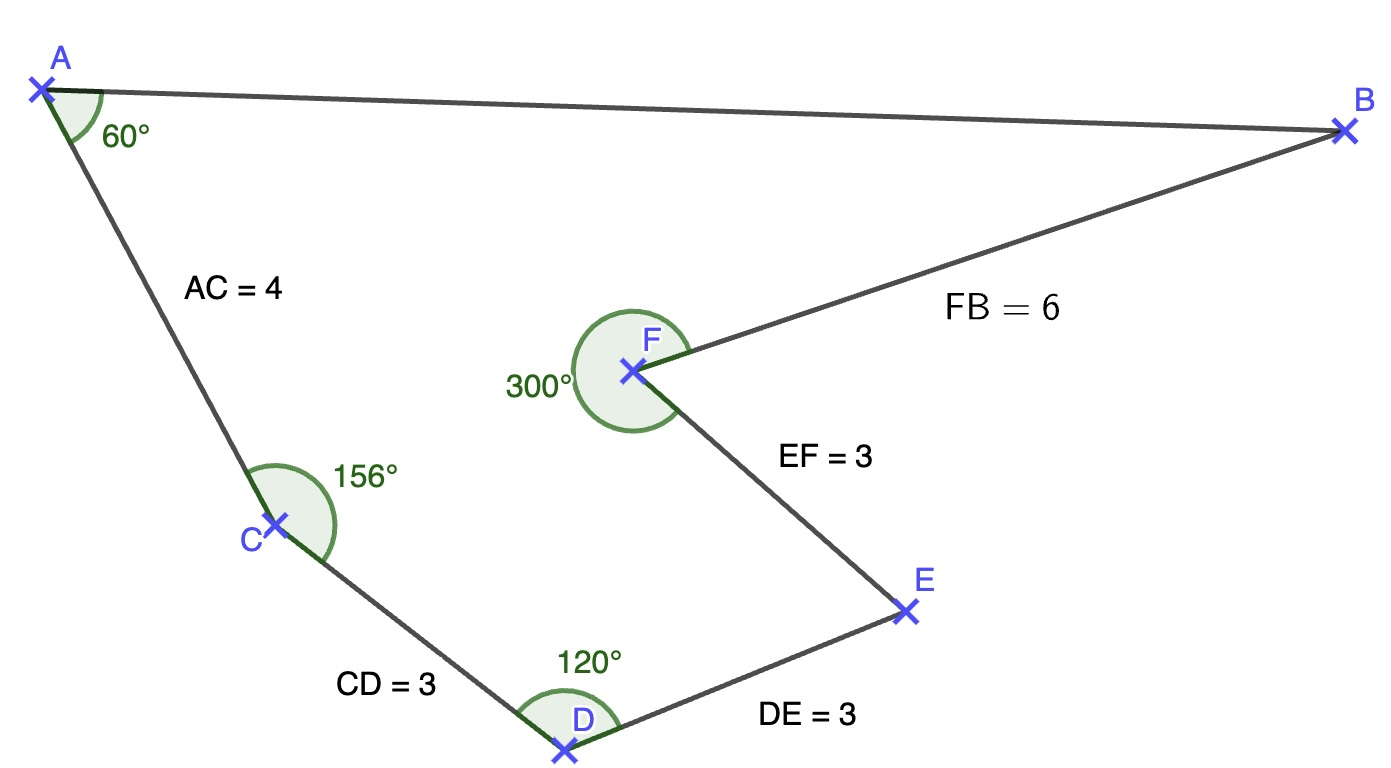
\includegraphics[width=15 cm]{Exo1.jpg}

\subsection*{Exercice 3 - 9 points}

\begin{enumerate}
\item{} [1 pt] Écrire une fraction dont le numérateur est égal à la somme du dénominateur et de $2$.
\item{} [1 pt] Trouver une fraction égale à $\frac53$ avec $25$ comme numérateur.
\item{} [2 pts] Simplifier le plus possible la fraction $\frac{84}{126}$. 
\item {} [1 pt] Réduire les fractions $\frac19$ et $\frac2{15}$ au même dénominateur.
\item{} [2 pts] Trier les fractions dans l'ordre décroissant $\frac25$, $\frac5{20}$ et $\frac{3}{10}$. 
\item{} [1 pt] Les fractions $\frac{13}{25}$ et $\frac{27}{52}$ sont-elles égales ? (Justifier). 
\item{} [1 pt] Montrer que les fractions $\frac{1~234}{9~434}$ et $\frac{1~392}{9~768}$ sont différentes.

\end{enumerate}



\end{document}